% !TEX TS-program = pdflatex
% !TEX encoding = UTF-8 Unicode

% This is a simple template for a LaTeX document using the "article" class.
% See "book", "report", "letter" for other types of document.

\documentclass[11pt]{article} % use larger type; default would be 10pt

\usepackage[utf8]{inputenc} % set input encoding (not needed with XeLaTeX)

%%% Examples of Article customizations
% These packages are optional, depending whether you want the features they provide.
% See the LaTeX Companion or other references for full information.

%%% PAGE DIMENSIONS
\usepackage{geometry} % to change the page dimensions
\geometry{a4paper} % or letterpaper (US) or a5paper or....
% \geometry{margin=2in} % for example, change the margins to 2 inches all round
% \geometry{landscape} % set up the page for landscape
%   read geometry.pdf for detailed page layout information

\usepackage{graphicx} % support the \includegraphics command and options

% \usepackage[parfill]{parskip} % Activate to begin paragraphs with an empty line rather than an indent

%%% PACKAGES
\usepackage{tikz}
\usepackage{booktabs} % for much better looking tables
\usepackage{color} % Added by me
\usepackage{array} % for better arrays (eg matrices) in maths
\usepackage{paralist} % very flexible & customisable lists (eg. enumerate/itemize, etc.)
\usepackage{verbatim} % adds environment for commenting out blocks of text & for better verbatim
\usepackage{subfig} % make it possible to include more than one captioned figure/table in a single float
% These packages are all incorporated in the memoir class to one degree or another...

%%% HEADERS & FOOTERS
\usepackage{fancyhdr} % This should be set AFTER setting up the page geometry
\pagestyle{fancy} % options: empty , plain , fancy
\renewcommand{\headrulewidth}{0pt} % customise the layout...
\lhead{}\chead{}\rhead{}
\lfoot{}\cfoot{\thepage}\rfoot{}

%%% SECTION TITLE APPEARANCE
\usepackage{sectsty}
\allsectionsfont{\sffamily\mdseries\upshape} % (See the fntguide.pdf for font help)
% (This matches ConTeXt defaults)

%%% ToC (table of contents) APPEARANCE
\usepackage[nottoc,notlof,notlot]{tocbibind} % Put the bibliography in the ToC
\usepackage[titles,subfigure]{tocloft} % Alter the style of the Table of Contents
\renewcommand{\cftsecfont}{\rmfamily\mdseries\upshape}
\renewcommand{\cftsecpagefont}{\rmfamily\mdseries\upshape} % No bold!

%%% END Article customizations

%%% The "real" document content comes below... %%%

\title{Variation of Tournaments}
\author{Ethan Schaffer}
\date{Due 10/18/16}
\newcommand\tab[1][1cm]{\hspace*{#1}}

\begin{document}
\maketitle

\section{Problem}
How many tournaments on n vertices are there?

\section{Solution}
To solve this problem, I used what I learned from 4.8.7, 4.8.8, 4.8.9, and 4.8.10. 

\subsection*{Problem 4.8.7}
\textit{Notice that the sum of scores in the example in Figure 4.33 is 10. Give another example of a tournament with five teams. What is its score vector?}\\
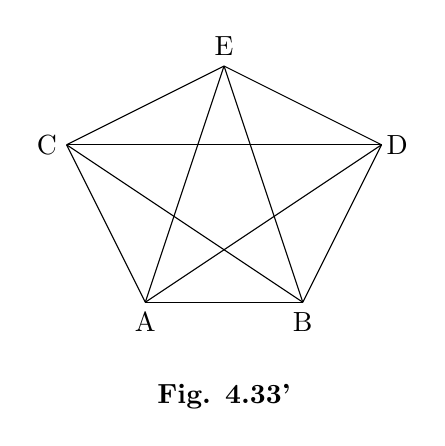
\begin{tikzpicture}
\draw (0, -.25) node {A};
\draw (2, -.25) node {B};
\draw (-1.25, 2) node {C};
\draw (3.2, 2) node {D};
\draw (1, 3.25) node {E};

\draw (0,0) -- (2,0); %AB
\draw (0,0) -- (-1,2); %AC
\draw (0,0) -- (3,2); %AD
\draw (0,0) -- (1,3); %AE
\draw (2,0)--(-1, 2); %BC
\draw (2,0)--(3, 2); %BD
\draw (2,0)--(1, 3); %BE
\draw (-1, 2)--(3, 2); %CD
\draw (-1, 2)--(1, 3); %CE
\draw (3, 2)--(1, 3); %DC

\draw (1, -1.2) node {$\textbf{Fig. 4.33'}$};
\end{tikzpicture}

\textit{What is the sum of the scores?}\\ 
\tab The sum of figure 4.33' is also 10. \\

\textit{What is the sum of the scores for a tournament with n teams?}\\
\tab The sum of the score for a tournment is equal to its number of edges. Therefore, it is equal to $\frac{(n)(n-1)}{2}$.\\

\textit{What is the largest possible score?} \\
\tab The largest possible score a single team can have is if it beats all of it's opponents. \\
\tab Therefore, that score is n-1.

\subsection*{Problem 4.8.8}
\textit{Show that \{0, 1, 2, . . . , n - 1\} is the score vector of some transitive tournament with n teams.}
\\ \tab The score vector of figure 4.33 is \{0, 1, 2, 3, 4\} when it is sorted to bee \{A, B, C, D, E\}.

\subsection*{Problem 4.8.9}
\textit{Suppose T is a transitive tournament. Show that the score vector of T \textbf{cannot} have two equal values. Hint: Suppose two teams, A and B, have equal scores. Suppose A beats B. Now suppose B beats C.} \\
\textit{Can C beat A?}
\\ \tab C cannot beat A, because if that happened T would be become a transitive tournament.

\textit{Can every team that B beats beat A? Why not?}
\\ \tab No, because then there would be a directed 3 cycle between A, B, and that team (K).

\textit{Conclude that A must beat all the teams that B beats. Why is this not possible?}
I used a proof by contradiction to show that it is impossible to have K beat A. If K did, then A, B, and C would have the same number of wins. If A beats K, then A and B would have a different number of wins. 
\\ \tab 

\subsection*{Problem 4.8.10}
\textit{Conclude from Exercise 4.8.9 that if T is a transitive tournament on n teams, 
then the score vector of T must be some rearrangement of \{0, 1, 2, . . . , n - 1\}.}
\\ \tab We know that in every transitive tournament, one team beats everyone. That team has number of wins of \textit{n-1}. One team has to win against all teams except for that one, so it has \textit{n-2} wins. Every team would have some number of wins between \textit{0 and n-1}. Another way of reaching this conclusion is from what I have already shown. We know that every team must have a different number of wins, and they must sum up to \begin{displaymath}((n)(n-1))/2\end{displaymath}
This can only be accomplished if we have a list of \{0, 1, 2, . . . , n - 1\}. 

\subsection*{How many tournments on n vertices are there?}
\tab I already know from 4.8.10 that the score vector of T must always be some rearrangement of \{0, 1, 2, . . . , n - 1\}. Therefore, I knew that I can put the n terms of the vertor into any order. Using factorials (notated as !) is a very simple way to model the nubmber of possibilities. So, I know that the formula would involve n!, where n! is the number of possible score vectors. However, I also know that I can flip over every arrow of the tournament and maintain T's transitivity. So, I am pretty sure that the final equation would be 
\begin{displaymath} T(n) = 2n! \end{displaymath} 
\tab However, I thought that the 2 at  the front of that might not be needed. The question really is whether or not the flipped version could already be found in another variation. After trying some examples of T(3), T(4), etc, I realized that I didn't need to 2 after all. So, I conclude that \begin{displaymath} T(n)=n! \end{displaymath}

\subsection*{Analysis}
\tab This problem was very interesting, and a lot of fun to figure out. The relationships between 

\subsection*{Status}
\tab I feel like I understand most of this problem, but I couldn't completely understand the end conclusion of 4.8.10. Otherwise, I felt like I understood and explained everything very well. 

\subsection*{MVP}
\tab I have no MVP for this problem.

\end{document}
